% 图片使用了subfigure环境
% 表格都改为了 lstlisting环境
% 协整部分增加了解释
% 本节中所有的英文标点替换为中文标点
% 修正了其它的一些小错误
% ----------------------------------
% 修改了表格的排版
% ----------------------------------

\section{与退休养老资产的协整关系}
由于美国FOF基金的兴起, 主要源于养老金市场的发展。 美国雇员逐渐选择将养老金计划由DB(Defined Benefit) Plan转向DC(Defined Contribute) Plan, 增大了养老金投资着的投资需求。 而FOF基金作为一种收益稳定、风险二次分散的基金, 自然受到了这些被动投资者的青睐。 下面, 利用彭博数据库中FOF基金资产总量和养老金资产总量的季度数据, 对FOF基金市场与养老金市场进行协整分析。 在2007--2016十年中, 二者的绝对数量和增长率变化趋势如图~\ref{pic:3-0}~:



\begin{figure}[h!]
	\begin{minipage}[ht]{0.47\textwidth}
		\centering
		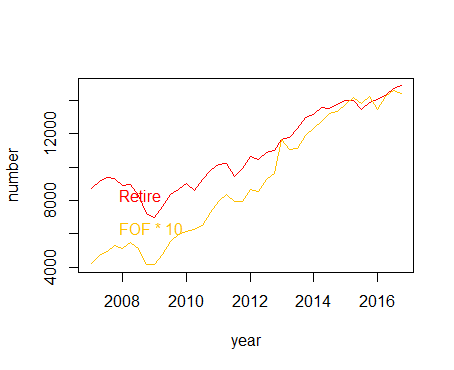
\includegraphics[width=1\textwidth]{pic/3-0-1.png}
		\subcaption{}\label{pic/3-0-1.png}
	\end{minipage}%
	\hspace{0.06\textwidth}
	\begin{minipage}[ht]{0.47\textwidth}
		\centering
		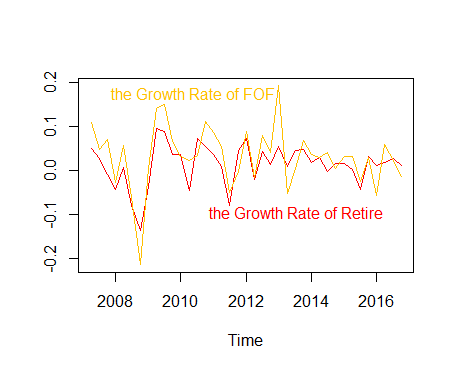
\includegraphics[width=1\textwidth]{pic/3-0-2.png}
		\subcaption{}\label{pic/3-0-2.png}
	\end{minipage}
	\caption{2007-2016年FOF基金和养老金发展情况季度数据:(a)1资产数量;(b)资产增长率} \label{pic:3-0}
\end{figure}





% 单位根检验部分
对$\{FOF_t\}$和${Retire_t}$序列分别进行单位根检验。ADF检验和Phillips–Perron的结果接受了原假设(单位根过程), 并且Kwiatkowski–Phillips–Schmidt–Shin检验结果拒绝了原假设(平稳过程)。 因此可以认为${FOF_t}$和${Retire_t}$是非平稳序列。
继续对它们的差分序列${\Delta FOF_t}$和${\Delta Retire_t}$进行单位根检验, 得到的结果表明它们是平稳序列。 所以, ${FOF_t}$和${Retire_t}$分别是2个$I(1)$序列。下面对这两个序列进行协整估计。

% 单位根检验表格
\begin{framed}
\begin{verbatim}
 *---------------------------------*                         
 *          Unit Root Test         *                           
 *---------------------------------*
TEST Method      ADF       KPSS      PP  
FOF             2.53       1.07   -1.06
diff(FOF)      -3.40       0.11   40.00
Retire          1.64       1.01    0.23
diff(Retire)   -2.31       0.18    1.55
10pct          -1.61       0.35     *  
5pct           -1.95       0.46    0.26
1pct           -2.62       0.74     *  
\end{verbatim}
\end{framed}


% 协整部分
首先, 使用最小二乘法估计如下方程:
$$FOF_t = \alpha + \beta \cdot Retire_t + \mu_t$$
得到$\alpha$和$\beta$的估计量$\hat{\alpha}$和$\hat{\beta}$。 估计结果如下表所示。

% OLS回归结果表格
\begin{framed}
\begin{verbatim} 
Call:
lm(formula = fof ~ retire)

Residuals:
     Min       1Q   Median       3Q      Max 
-182.482  -26.622    1.348   38.330  145.811 

Coefficients:
              Estimate Std. Error t value Pr(>|t|)    
(Intercept) -7.552e+02  5.632e+01  -13.41 5.51e-16 ***
retire       1.524e-01  5.042e-03   30.22  < 2e-16 ***
---
Signif. codes:  0 '***' 0.001 '**' 0.01 '*' 0.05 '.' 0.1 ' ' 1

Residual standard error: 74.18 on 38 degrees of freedom
Multiple R-squared:  0.9601,    Adjusted R-squared:  0.959 
F-statistic: 913.5 on 1 and 38 DF,  p-value: < 2.2e-16
\end{verbatim}
\end{framed}



对残差估计序列${\hat{\mu}_t}$进行单位根检验, ${\hat{\mu}_t}$在ADF检验和PP检验中拒绝了存在单位根的原假设, 在KPSS检验中接受了序列平稳的原假设。因此可以认为${FOF_t}$和${Retire_t}$两个$I(1)$过程得到了平稳的$I(0)$
过程。 即两个序列之间存在着长期的均衡关系(协整关系)。 协整向量为$(1, -0.15)$。

% 残差具有平稳性
\begin{framed}
\begin{verbatim}
 *---------------------------------------------------------*
 *                      Unit Root Test                     *
 *---------------------------------------------------------*    
TESTs             ADF-Test       KPSS-Test           PP-Test
Statistics   -3.18 (<1pct)   0.27 (<10pct)   -10.04 (<Z-tau)
\end{verbatim}
\end{framed}

% Error Correction Model
记$y_t = FOF_t$, $x_t = Retire_t$, 建立误差修正模型。 由于使用的是季度数据, 所以加入$\Delta y_t$的1--4阶滞后项。
$$
\Delta y_t = \alpha_1 \cdot \Delta y_{t-1} + \alpha_2  \cdot \Delta  y_{t-2} + \alpha_3 \cdot \Delta  y_{t-3} + \alpha_4 \cdot \Delta  y_{t-4} + \beta_0 \cdot \Delta  x_t+\beta_1 \cdot \Delta  x_{t-1} + \gamma \cdot ( y_{t-1}-kx_{t-1}) + \epsilon_t
$$


估计结果如下表所示:

% 误差修正模型的估计结果
\begin{framed}
\begin{verbatim}
 *---------------------------------------------------------*
 *                 Error Correction Model                  *
 *---------------------------------------------------------* 
Call:
dynlm(formula = y ~ L(y, 1) + L(y, 2) + L(y, 3) + L(y, 4) + L(x, 
    1) + L(x, 0) + L(r, 1), data = ecmdat1)

Residuals:
    Min      1Q  Median      3Q     Max 
-87.387 -20.436   1.006  16.815 142.580 

Coefficients:
            Estimate Std. Error t value Pr(>|t|)    
(Intercept) 22.13335   11.14436   1.986   0.0573 .  
L(y, 1)     -0.46108    0.19994  -2.306   0.0290 *  
L(y, 2)     -0.01601    0.12908  -0.124   0.9022    
L(y, 3)     -0.03563    0.12999  -0.274   0.7861    
L(y, 4)     -0.02875    0.13862  -0.207   0.8373    
L(x, 1)      0.05842    0.02549   2.292   0.0300 *  
L(x, 0)      0.09517    0.01852   5.138  2.1e-05 ***
L(r, 1)     -0.38373    0.16855  -2.277   0.0309 *  
---
Signif. codes:  0 '***' 0.001 '**' 0.01 '*' 0.05 '.' 0.1 ' ' 1

Residual standard error: 40.94 on 27 degrees of freedom
Multiple R-squared:  0.5683,    Adjusted R-squared:  0.4564 
F-statistic: 5.078 on 7 and 27 DF,  p-value: 9e-04
\end{verbatim}
\end{framed}


协整方程的估计结果为
$$\Delta y_t =22.13  -0.46 \cdot \Delta y_{t-1} -0.01 \cdot \Delta  y_{t-2}   -0.04 \cdot \Delta  y_{t-3}  -0.03 \cdot \Delta  y_{t-4} + 0.10 \cdot \Delta  x_t+ 0.06 \cdot \Delta  x_{t-1} -0.38 \cdot ( y_{t-1}-0.15x_{t-1}) + \epsilon_t$$
$\Delta y$的滞后项中,只有一期滞后项是显著的;误差修正项的系数为-0.38,在10\%的程度显著,符合反向修正机制。 协整向量为$(1, -0.15)$。
ECM模型说明FOF基金市场和养老金市场存在长期的稳定关系(图~\ref{fg:coin-result}~)。从资产数量的角度上,养老金市场的发展推动了FOF基金市场的发展;长期均衡中,FOF基金的资产总量维持在养老金市场资产总量的15\%。而上一期的不均衡误差对当期以38\%的比率进行修正。

\begin{figure}[h!]
  \centering
  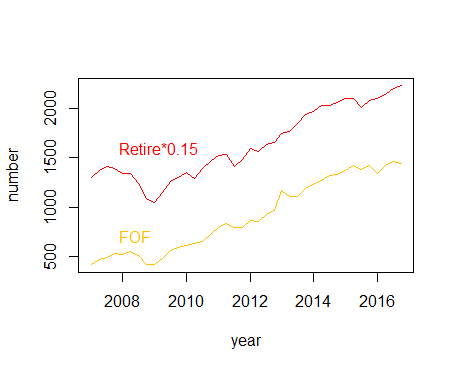
\includegraphics[width=0.6\textwidth]{pic/coin-result.png}
  \caption{长期均衡关系}\label{fg:coin-result}
\end{figure}

美国养老金体系包括政府主办的退休金保险、雇主资助的私营养老金、个人储蓄多个层次。从DB Plan(确定收益计划)到DC Plan(确定退休金计划)的演变,使得雇员更多地考虑到投资工具的收益的稳定性。
而共同基金,特别是FOF是养老金的理想投资工具。和其它投资工具相比,FOF基金具有一些天然的投资优势:(1)低风险性,基金本身通过组合的方式,对股票和证券进行了资产分散;而FOF基金则通过投资不同类型基金,进行双重的风险分散,从而能够获得更加稳定的收益;(2)降低了多样化投资门槛,投资者不再需要繁复地挑选基金,可以通过只投资一个产品来获得相似的投资效果。

借鉴美国养老金与FOF市场的关联关系的实证经验,可以对中国市场得到启示。2016年末,中国社保基金资产总额达到20,423.28亿元。而中国社会提前进入老龄化社会,使得养老保险制度面临更大的挑战。
目前,中国资本市场还不成熟, 特别是股票市场波动较大,存在着资产质量报告及信息不对称、庄家操纵股价等一系列的问题 ,而且缺乏有效的避险工具。在这样的情况下,选择稳定收益的投资工具十分重要。
此外,由美国市场的经验,养老金市场的发展也在推动了FOF基金的发展。养老金成熟的投资于FOF基金,也会促进FOF基金的发展,进而推动共同基金市场的发展。
